%!TEX root = ../main.tex

\chapter{Experimental Setup}	\label{ch::experimental_setup}
\chaptermark{Experimental Setup}

	I this chapter, the experimental setups which are used for the of the experiments described in this thesis will be introduced. 
	The key measurements of this thesis are fluorescence measurements of \sivs in nanodiamonds.
	For this aim, a home-built confocal setup is used, which is described in the first part of this chapter.
	A slightly modified version of the setup is used to perform measurements of the Raman emission of the diamond host material, described in the second part of this chapter.
	The last part describes a completely different setup, which is used to transfer \nds from the original substrate to other photonic structures.




	\section{Confocal Setup}

	The confocal setup serves to perform a series of measurement of fluorescence light: scanning the sample to find \sivs, recording luminescence spectra of the aforementioned, determine the saturation count rate and determine whether the emitter in question is a single emitter by performing photon autocorrelation measurements.
	The two key components for these measurements are 

	\begin{itemize}
		\item A Hanbury-Brown and Twiss setup to investigate the single photon character. It is built up of two avalanche photo diodes (APDs) which also serve to scan the sample in order to find emitters on the sample surface; and to perform saturation measurements.
		\item A spectrometer to investigate the spectral properties.
	\end{itemize}


	\begin{figure}[t] %fig::confocal_setup
		\centering
		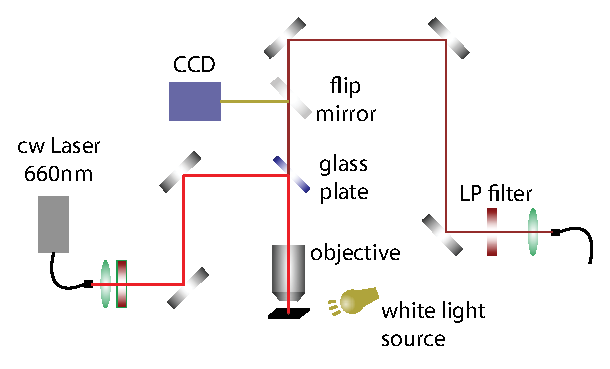
\includegraphics[width=\linewidth]{./pics/confocal_setup.eps}
		\caption{Confocal setup}
		\label{fig::confocal_setup}
	\end{figure}

	\begin{figure}[t] %fig::hbt_spectrometer
		\centering
		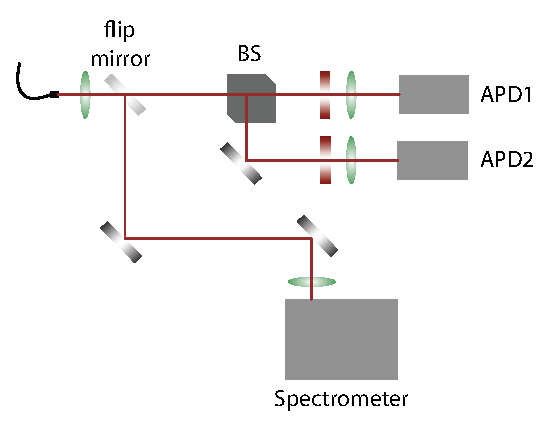
\includegraphics[width=\linewidth]{./pics/hbt_spectrometer.eps}
		\caption{HBT, spectrometer}
		\label{fig::hbt_spectrometer}
	\end{figure}

	\autoref{fig::confocal_setup} depicts a sketch of the confocal setup. 
	Except for the laser and the sample stage, the whole setup is fixed to a vertical breadboard. 
	This design allows for easy exchanging of the samples, without the need of gluing them to a vertical stage.

	The friction between the sample and the aluminum surface of the stage is sufficient that the sample does not move during scanning.
	If it is important that the sample has a a defined orientation, it is put inside of an aluminum angle.
	The stage is powered with two stepper motors (\todo{type}) in the horizontal x and y directions.
	The objective is fixed to another stage which in turn is fixed to the vertical breadboard.
	In this way, the vertical z direction is implemented for focusing the laser light on the sample.

	The bright red color at the left-hand side of the sktech represents the excitation beam path.
	The sample is excited with a continuous wave diode laser (Sch\"after-Kirchhoff, 58FCM) which emits at a wavelength of \SI{660}{\nano\meter}.
	The outlet of the light is through a pigtail fiber, the light is outcoupled and collimated exploiting an aspheric lens.
	To suppress sideband emission from the laser, a bandpass filter with a window of  \SI{10}{\nm} around a center of \SI{660}{\nm} is used.
	The excitation beam then hits a beamsplitter (described below) and is guided through the objective (numerical aperture of 0.8, Olympus, LMPlanFLN 100x) and focused on the sample.

	As the luminescence light from the emitter is in the same focus as the excitation laser light, it is effectively collected by the objective.
	Hence also the name confocal setup.

	The collected light then follows the detection beam path depicted in a dark red color in \autoref{fig::confocal_setup}.
	First, it passes through the beamsplitter.
	According to the experimental necessities, either a \todo{thickness} glass plate (fabricator Halle Germany) with a transmission of 90\% or a dichroic mirror is employed.
	While the glass plate features a higher collection efficiency and therefore, more of the fluorescence light is detected, the dichroic mirror allows for a higher excitation intensity using the same excitation laser. 
	However, a high excitation intensity may cause permanent fluorescence intermittence of the \sivs (for further detail, refer to \todo{insert chapter}).
	In general, if a high excitation is necessary, for instance for saturation measurements \todo{saturation already introduced?}, 


	\section{Raman Measurements}
	\section{Nanomanipulator}

